% Provenance (never printed): see sources/outline_sources.md (Year 1: crystal
% chemistry of minerals, silicates, solid solutions, mineral formulas, the main
% rock-forming minerals). Olivine curves in figdata/bachelor-1/solid_solution.py;
% the olivine analysis of the problem is invented (Fo about 82); exercise and
% problem values in the Book 3 scratch calculator calc/ch07.py.
\chapter{Les minéraux des roches}\label{ch:b1:rock-forming-minerals}

Un plan de travail en granite montre trois ou quatre sortes de grains~: du
quartz gris vitreux, du \omterm{def:b1:rock-forming-minerals:groups}{feldspath} rose ou blanc, des paillettes de \omterm{def:b1:rock-forming-minerals:groups}{mica} noir. Un
sable de plage est presque entièrement du quartz. Les petits cristaux verts
dispersés dans un basalte sont de l'\omterm{def:b1:rock-forming-minerals:groups}{olivine}, et le même \omterm{def:b1:rock-forming-minerals:mineral}{minéral}, de composition
légèrement différente, forme l'essentiel du manteau supérieur. Une poignée de
minéraux construit presque toutes les roches, et presque tous sont des
silicates~: de l'oxygène et du silicium, les deux éléments les plus abondants de
la croûte, réunis en tétraèdres qui s'enchaînent de quelques façons simples. Ce
chapitre explique comment l'enchaînement fixe la formule et l'habitus d'un
silicate, comment un élément en remplace un autre dans un cristal de sorte qu'un
\omterm{def:b1:rock-forming-minerals:mineral}{minéral} est une gamme de compositions plutôt qu'une seule, comment une analyse
chimique devient une formule, et quels sont les principaux minéraux des roches.
Il se termine par une \omterm{def:b1:rock-forming-minerals:groups}{olivine} de basalte, analysée, recalculée et pesée.

\begin{recall}
Un cristal est un solide dont les atomes se répètent sur un réseau~; la maille
est la plus petite boîte qui se répète, et la coordinence d'un ion compte ses
plus proches voisins de charge opposée (chimie, volume de première année). Les
rayons ioniques dépendent de la charge et de la coordinence. Un \omterm{def:b1:rock-forming-minerals:mineral}{minéral}
s'identifie à la main par son habitus, son clivage, sa dureté et son éclat
(livre~2, année~11). La quantité de matière se compte en moles, et une masse
molaire est la masse d'une mole (chimie).
\end{recall}

\section{Ce qu'est un minéral}

\begin{definition}[Minéral]\label{def:b1:rock-forming-minerals:mineral}
Un \emph{minéral}\index{mineral@minéral} est un solide d'origine naturelle de structure cristalline définie
et de composition chimique soit fixe, soit variable dans des limites définies.
Presque tous les minéraux sont inorganiques.
\end{definition}

Une roche, au contraire, est un agrégat de grains d'un ou de plusieurs minéraux
(ou de verre)~: le granite est du quartz, des \omterm{def:b1:rock-forming-minerals:groups}{feldspaths} et du \omterm{def:b1:rock-forming-minerals:groups}{mica}~; le calcaire
est surtout de la calcite. Les deux moitiés de la définition sont indépendantes.
Le verre à vitre a la composition d'un silicate mais pas de structure
cristalline~: ce n'est pas un \omterm{def:b1:rock-forming-minerals:mineral}{minéral}, pas plus que le verre d'une lave trempée.
Inversement, une même composition peut cristalliser dans plusieurs structures, et
chaque structure est un \omterm{def:b1:rock-forming-minerals:mineral}{minéral} différent.

\begin{definition}[Polymorphe]\label{def:b1:rock-forming-minerals:polymorph}
Deux minéraux sont des \emph{polymorphes}\index{polymorphe} l'un de l'autre lorsqu'ils ont la même
composition chimique et des structures cristallines différentes.
\end{definition}

Le carbone cristallise en graphite, un empilement de feuillets d'hexagones de
masse volumique \qty{2.16}{g.cm^{-3}}, et en diamant, une charpente où chaque
atome a quatre voisins, de masse volumique \qty{3.51}{g.cm^{-3}}. Le carbonate de
calcium est de la calcite (\qty{2.71}{g.cm^{-3}}) ou de l'aragonite
(\qty{2.93}{g.cm^{-3}})~; la silice est du quartz (\qty{2.65}{g.cm^{-3}}) ou de la
coésite (\qty{2.93}{g.cm^{-3}})~; \ce{Al2SiO5} est du disthène
(\qty{3.61}{g.cm^{-3}}), de l'andalousite (\qty{3.15}{g.cm^{-3}}) ou de la
sillimanite (\qty{3.24}{g.cm^{-3}}).
% ledger: webmineral:polymorphs, hom:calcite, hom:quartz
Dans chaque paire, le \omterm{def:b1:rock-forming-minerals:polymorph}{polymorphe} le plus dense est celui qui se forme à plus
haute pression~: à une température donnée, une élévation de la pression favorise
l'état de plus petit volume (chimie, déplacement d'un équilibre). Le diamant
d'une kimberlite et la coésite d'une roche frappée par une météorite enregistrent
donc des pressions que l'on ne trouve que profondément dans le manteau ou lors
d'un impact. Les trois \omterm{def:b1:rock-forming-minerals:polymorph}{polymorphes} de \ce{Al2SiO5}, dont les domaines de
stabilité se partagent le plan pression--température, servent à lire les
conditions du métamorphisme (volume de deuxième année).

\section{Le tétraèdre silicaté et ses enchaînements}

Dans tout silicate courant, chaque atome de silicium occupe le centre de quatre
atomes d'oxygène placés aux sommets d'un tétraèdre régulier~: l'unité
\ce{SiO4} rappelée de la chimie. L'ion silicium est petit
(\qty{0.26}{\angstrom} en coordinence quatre) et l'ion oxyde gros, si bien que
quatre oxygènes tiennent autour de lui et pas davantage~; la liaison
silicium--oxygène est forte et en partie covalente. Une unité isolée porte une
charge $4 - 4\times2 = -4$.
% ledger: shannon:radii
Les tétraèdres peuvent être isolés, leur charge compensée par des cations
métalliques placés entre eux, ou partager des sommets~: un oxygène commun à deux
tétraèdres est un oxygène \emph{pontant}. Deux tétraèdres ne partagent jamais une
arête ni une face, ce qui rapprocherait trop deux siliciums. Les silicates se
classent d'après le nombre de sommets que chaque tétraèdre partage
(\cref{def:b1:rock-forming-minerals:silicate-classes}).

\begin{omfigure}
\tikzset{
  tup/.pic={\filldraw[fill=omLithLime, draw=black, line join=round] (0,0) -- (1,0) -- (0.5,0.866) -- cycle;
            \fill[omThm] (0.5,0.2887) circle (0.11);},
  tdn/.pic={\filldraw[fill=omLithLime, draw=black, line join=round] (0,0) -- (1,0) -- (0.5,-0.866) -- cycle;
            \fill[omThm] (0.5,-0.2887) circle (0.11);},
  linkpanel/.style={x=0.45cm, y=0.45cm, baseline=(current bounding box.south)}}
\setlength{\tabcolsep}{4pt}
\begin{tabular}{cccc}
% (a) the tetrahedron in perspective
\begin{tikzpicture}[linkpanel]
  \useasboundingbox (-1.2,-1.0) rectangle (6.0,4.4);
  \coordinate (T) at (2.2,3.7); \coordinate (L) at (0.3,0.5); \coordinate (R) at (4.1,0.1);
  \coordinate (B) at (3.3,2.1); \coordinate (C) at (2.475,1.6);
  \draw[densely dashed, gray] (L) -- (B) -- (R) (B) -- (T);
  \shade[ball color=omLithShale] (B) circle (0.42);
  \draw[gray] (C) -- (T) (C) -- (L) (C) -- (R) (C) -- (B);
  \shade[ball color=omThm!70] (C) circle (0.24);
  \draw[thick, line join=round] (T) -- (L) -- (R) -- cycle;
  \foreach \p in {T,L,R} \shade[ball color=omLithShale] (\p) circle (0.42);
  \node[right] at (4.5,0.1) {\scriptsize O};
  \node[right] at (2.6,3.8) {\scriptsize O};
  \draw[omThm] (C) -- (4.6,2.2) node[right] {\scriptsize Si};
\end{tikzpicture} &
% (b) nesosilicate: isolated tetrahedra
\begin{tikzpicture}[linkpanel]
  \useasboundingbox (-1.2,-1.0) rectangle (6.0,4.4);
  \pic at (0,0.3) {tup}; \pic at (2.4,0.3) {tup}; \pic at (4.0,1.9) {tdn};
  \pic at (1.2,2.4) {tdn}; \pic at (3.0,2.8) {tup};
\end{tikzpicture} &
% (c) sorosilicate: pairs
\begin{tikzpicture}[linkpanel]
  \useasboundingbox (-1.2,-1.0) rectangle (6.0,4.4);
  \pic at (0,0.9) {tup}; \pic at (1,0.9) {tdn};
  \pic at (2.6,2.6) {tup}; \pic at (3.6,2.6) {tdn};
\end{tikzpicture} &
% (d) cyclosilicate: a ring of six
\begin{tikzpicture}[linkpanel]
  \useasboundingbox (-1.2,-1.0) rectangle (6.0,4.4);
  \begin{scope}[shift={(2.4,1.7)}]
  \foreach \t in {0,60,...,300} {
    \filldraw[fill=omLithLime, draw=black, line join=round] (\t-30:1) -- (\t+30:1) -- (\t:1.732) -- cycle;
    \fill[omThm] (\t:1.155) circle (0.11);}
  \end{scope}
\end{tikzpicture} \\
{\small (a) le tétraèdre \ce{SiO4}} & {\small (b) \omterm{def:b1:rock-forming-minerals:silicate-classes}{nésosilicate}} & {\small (c) \omterm{def:b1:rock-forming-minerals:silicate-classes}{sorosilicate}} & {\small (d) \omterm{def:b1:rock-forming-minerals:silicate-classes}{cyclosilicate}} \\
 & {\scriptsize $s = 0$, \ce{SiO4}} & {\scriptsize $s = 1$, \ce{Si2O7}} & {\scriptsize $s = 2$, \ce{Si6O18}} \\[6pt]
% (e) single chain
\begin{tikzpicture}[linkpanel]
  \useasboundingbox (-0.6,-1.2) rectangle (7.6,4.6);
  \begin{scope}[shift={(0,1.5)}]
  \foreach \i in {0,...,3} \pic at (2*\i,0) {tup};
  \foreach \i in {0,...,2} \pic at (2*\i+1,0) {tdn};
  \end{scope}
\end{tikzpicture} &
% (f) double chain: two single chains joined through every other apex
\begin{tikzpicture}[linkpanel]
  \useasboundingbox (-0.6,-1.2) rectangle (7.6,4.6);
  \begin{scope}[shift={(0.5,0.4)}]
  \foreach \i in {0,...,3} {\pic at (2*\i,0) {tup}; \pic at (2*\i,1.732) {tdn};}
  \foreach \i in {0,...,2} {\pic at (2*\i+1,0) {tdn}; \pic at (2*\i+1,1.732) {tup};}
  \end{scope}
\end{tikzpicture} &
% (g) sheet
\begin{tikzpicture}[linkpanel]
  \useasboundingbox (-0.6,-1.2) rectangle (7.6,4.6);
  \foreach \j in {0,1,2} {
    \foreach \i in {0,1,2} {\pic at (2*\i+\j,1.732*\j) {tup};}
    \foreach \i in {0,1} {\pic at (2*\i+\j+1,1.732*\j) {tdn};}}
\end{tikzpicture} &
% (h) framework: a sheet whose apices point alternately up and down
\begin{tikzpicture}[linkpanel]
  \useasboundingbox (-0.6,-1.2) rectangle (7.6,4.6);
  \foreach \j in {0,1,2} {
    \foreach \i in {0,1,2} {\pic at (2*\i+\j,1.732*\j) {tup};}
    \foreach \i in {0,1} {\pic at (2*\i+\j+1,1.732*\j) {tdn};}}
  \foreach \j in {0,1,2} \foreach \i in {0,1} {
    \filldraw[fill=white, draw=omThm, thick] (2*\i+\j+1.5,1.732*\j-0.2887) circle (0.17);}
\end{tikzpicture} \\
{\small (e) chaîne simple} & {\small (f) chaîne double} & {\small (g) feuillet} & {\small (h) charpente} \\
{\scriptsize $s = 2$, \ce{SiO3}} & {\scriptsize $s = 2$ et $3$, \ce{Si4O11}} & {\scriptsize $s = 3$, \ce{Si2O5}} & {\scriptsize $s = 4$, \ce{SiO2}} \\
\end{tabular}
\medskip

{\small Le tétraèdre \ce{SiO4} (a) et les façons dont les tétraèdres se lient,
vus de dessus~: chaque triangle est la base d'un tétraèdre, avec trois oxygènes à
ses sommets, le quatrième au-dessus du point, qui marque le silicium. Les sommets
qui se touchent sont des oxygènes partagés~; $s$ est le nombre de sommets que
partage chaque tétraèdre. Dans la charpente (h), les oxygènes apicaux (cercles
ouverts~: pointant vers le bas~; points~: pointant vers le haut) sont eux aussi
partagés, avec les feuillets du dessous et du dessus.}
\end{omfigure}

\begin{definition}[Les classes de silicates]\label{def:b1:rock-forming-minerals:silicate-classes}
Les silicates se classent d'après l'enchaînement de leurs tétraèdres \ce{SiO4}.
Dans un \emph{nésosilicate}\index{nesosilicate@nésosilicate}, les tétraèdres sont isolés~; dans un
\emph{sorosilicate}\index{sorosilicate}, ils sont liés par paires par un oxygène
partagé~; dans un \emph{cyclosilicate}\index{cyclosilicate}, ils forment des
anneaux fermés, chacun partageant deux sommets~; dans un \emph{inosilicate}\index{inosilicate},
ils forment des chaînes sans fin, simples (chaque tétraèdre partageant deux
sommets) ou doubles (deux chaînes simples jointes côte à côte, la moitié des
tétraèdres partageant trois sommets)~; dans un \emph{phyllosilicate}\index{phyllosilicate}, ils forment
des feuillets sans fin, chacun partageant trois sommets~; dans un
\emph{tectosilicate}\index{tectosilicate}, ils forment une charpente
tridimensionnelle, chacun partageant ses quatre sommets.
\end{definition}

\begin{proposition}[Le rapport silicium/oxygène]\label{prop:b1:rock-forming-minerals:si-o}
Si chaque tétraèdre \ce{SiO4} d'un silicate partage en moyenne $s$ de ses quatre
sommets avec d'autres tétraèdres, et si chaque oxygène partagé appartient à
exactement deux tétraèdres, alors le réseau silicaté contient $4 - s/2$ oxygènes
par silicium, et porte une charge de $s - 4$ par silicium.
\end{proposition}

\begin{proof}
On compte les oxygènes tétraèdre par tétraèdre. Un tétraèdre ayant $s_i$ sommets
partagés possède entièrement ses $4 - s_i$ oxygènes non partagés et la moitié de
chacun de ses $s_i$ oxygènes partagés, puisque chacun est compté de nouveau par
le tétraèdre voisin~: il apporte $4 - s_i + s_i/2 = 4 - s_i/2$ oxygènes. En
sommant sur $N$ tétraèdres et en divisant par $N$, on obtient $4 - s/2$ oxygènes
par silicium, $s$ étant la moyenne des $s_i$. Chaque silicium apporte une charge
$+4$ et chaque oxygène $-2$, donc la charge par silicium est
$4 - 2(4 - s/2) = s - 4$.
\end{proof}

La proposition donne aussitôt l'anion de chaque classe. Tétraèdres isolés
($s = 0$)~: \ce{SiO4^{4-}}. Paires ($s = 1$)~: $4 - 1/2 = 7/2$, soit
\ce{Si2O7^{6-}}. Anneaux et chaînes simples ($s = 2$)~: \ce{SiO3^{2-}}, écrit
\ce{Si6O18^{12-}} pour un anneau de six, \ce{Si2O6^{4-}} pour deux tétraèdres
d'une chaîne. Chaînes doubles (la moitié avec $s = 2$, la moitié avec $s = 3$,
donc $s = 5/2$)~: $4 - 5/4 = 11/4$, \ce{Si4O11^{6-}}. Feuillets ($s = 3$)~:
\ce{Si2O5^{2-}}. Charpentes ($s = 4$)~: \ce{SiO2}, neutre --- le quartz est une
charpente de silicium et d'oxygène seuls. Plus les tétraèdres partagent, plus la
charge à compenser est petite et moins il y a de cations métalliques~: l'\omterm{def:b1:rock-forming-minerals:groups}{olivine}
\ce{Mg2SiO4} a deux ions métalliques par silicium, un \omterm{def:b1:rock-forming-minerals:groups}{pyroxène} comme l'enstatite
\ce{Mg2Si2O6} un seul, le quartz aucun.

L'enchaînement façonne aussi le cristal. Un silicate en feuillets se clive
facilement entre ses feuillets, où les liaisons sont faibles~: les \omterm{def:b1:rock-forming-minerals:groups}{micas} se
débitent en minces paillettes flexibles. Les silicates en chaînes se clivent
parallèlement à leurs chaînes, selon deux plans faisant un angle fixé par
l'empilement des chaînes~: environ \ang{87} et \ang{93} dans les \omterm{def:b1:rock-forming-minerals:groups}{pyroxènes}, dont
les chaînes sont étroites, \ang{56} et \ang{124} dans les \omterm{def:b1:rock-forming-minerals:groups}{amphiboles}, dont les
chaînes doubles sont plus larges. Les deux angles de clivage, vus sur un cristal
brisé ou en \omterm{def:b1:field-lab-methods-1:thin-section}{lame mince}, sont la façon classique de distinguer les deux groupes.
% ledger: hom:diopside, hom:mg-hornblende

\section{Substitution ionique et solutions solides}

Un cristal est un ensemble de sites, et un site se définit par sa taille et par
la charge qu'il requiert, non par un élément. Un ion de taille et de charge
convenables peut prendre la place d'un autre dans le cristal en croissance, et
aucune roche n'est assez pure pour n'en fournir qu'un seul.

\begin{definition}[Substitution ionique, substitution couplée]\label{def:b1:rock-forming-minerals:substitution}
Une \emph{substitution ionique}\index{substitution ionique} est le remplacement, dans un site d'une structure
cristalline, d'un ion par un autre de rayon voisin, sans changement de la
structure. Une \emph{substitution couplée}\index{substitution couplee@substitution couplée} est un couple de substitutions sur deux sites
différents dont les changements de charge s'annulent, de sorte que le cristal
reste neutre.
\end{definition}

Deux règles empiriques, dues à Goldschmidt, disent quelles substitutions sont
possibles. Les rayons doivent être voisins~: la substitution est libre lorsqu'ils
diffèrent de moins de \qty{15}{\percent} environ, limitée entre 15 et
\qty{30}{\percent} environ, et rare au-delà. Les charges ne doivent pas différer
de plus d'une unité, et une différence de charge doit être compensée ailleurs
dans la structure. Dans le site de coordinence six de l'\omterm{def:b1:rock-forming-minerals:groups}{olivine}, \ce{Mg^{2+}}
(\qty{0.72}{\angstrom}) est remplacé librement par \ce{Fe^{2+}}
(\qty{0.78}{\angstrom}, \qty{8}{\percent} plus gros) et par \ce{Ni^{2+}}
(\qty{0.69}{\angstrom}), peu par \ce{Mn^{2+}}
(\qty{0.83}{\angstrom}), à peine par \ce{Ca^{2+}} (\qty{1.00}{\angstrom},
\qty{39}{\percent} plus gros).
Les règles sont des guides~: la température élargit le domaine possible, car un
cristal chaud tolère davantage de contrainte, ce qui explique qu'un \omterm{def:b1:rock-forming-minerals:mineral}{minéral} formé
à haute température contienne souvent davantage d'ions mal ajustés que le même
\omterm{def:b1:rock-forming-minerals:mineral}{minéral} formé à froid.
% ledger: goldschmidt:size, shannon:radii

\begin{definition}[Solution solide, pôle pur]\label{def:b1:rock-forming-minerals:solid-solution}
Une \emph{solution solide}\index{solution solide (minerale)@solution solide (minérale)} est un \omterm{def:b1:rock-forming-minerals:mineral}{minéral} dans lequel un ou plusieurs sites
structuraux sont occupés, dans des proportions qui varient continûment, par deux
ions ou davantage. Les \emph{pôles purs}\index{pole pur@pôle pur} d'une solution solide sont les
compositions à ses limites, chacune avec chaque site variable rempli par un seul
ion~; une composition intermédiaire est donnée par les fractions molaires des
pôles purs.
\end{definition}

L'\omterm{def:b1:rock-forming-minerals:groups}{olivine} est la \omterm{def:b1:rock-forming-minerals:solid-solution}{solution solide} entre la forstérite \ce{Mg2SiO4} (Fo) et la
fayalite \ce{Fe2SiO4} (Fa), complète d'un \omterm{def:b1:rock-forming-minerals:solid-solution}{pôle pur} à l'autre~: une \omterm{def:b1:rock-forming-minerals:groups}{olivine} dont
\qty{82}{\percent} des sites de coordinence six sont occupés par le magnésium et
\qty{18}{\percent} par le fer s'écrit $\text{Fo}_{82}$, ou
\ce{(Mg_{0.82}Fe_{0.18})2SiO4}. Le \omterm{def:b1:rock-forming-minerals:groups}{grenat}, le \omterm{def:b1:rock-forming-minerals:groups}{pyroxène}, l'\omterm{def:b1:rock-forming-minerals:groups}{amphibole} et le \omterm{def:b1:rock-forming-minerals:groups}{mica}
sont des \omterm{def:b1:rock-forming-minerals:solid-solution}{solutions solides} de la même façon. Les \omterm{def:b1:rock-forming-minerals:groups}{feldspaths} \omterm{def:b1:rock-forming-minerals:groups}{plagioclases} sont une
\omterm{def:b1:rock-forming-minerals:solid-solution}{solution solide} d'une autre sorte, entre l'albite \ce{NaAlSi3O8} (Ab) et
l'anorthite \ce{CaAl2Si2O8} (An). Le sodium et le calcium ont presque le même
rayon (\qty{1.02}{\angstrom} et \qty{1.00}{\angstrom} en coordinence six) mais des
charges différentes~; chaque calcium qui entre doit être accompagné d'un
aluminium remplaçant un silicium dans un tétraèdre~:
% ledger: shannon:radii
\[
  \mathrm{Na^{+}} + \mathrm{Si^{4+}} \;\rightleftharpoons\; \mathrm{Ca^{2+}} + \mathrm{Al^{3+}},
\]
une \omterm{def:b1:rock-forming-minerals:substitution}{substitution couplée} qui laisse inchangée la charge totale.
L'aluminium peut entrer dans un tétraèdre parce qu'il est assez petit
(\qty{0.39}{\angstrom} en coordinence quatre)~; c'est le remplaçant le plus
courant du silicium dans les silicates.

\begin{omfigure}
\begin{tikzpicture}[x=1cm, y=1cm,
  site/.style={draw, minimum width=1.25cm, minimum height=0.75cm, font=\small},
  asite/.style={site, fill=omLithGranite!60},
  tsite/.style={site, fill=omLithLime}]
\node[font=\small\bfseries, anchor=east] at (-0.4,1.6) {albite};
\node[asite] (a0) at (0.5,1.6) {$\mathrm{Na^{+}}$};
\node[tsite] (a1) at (2.2,1.6) {$\mathrm{Al^{3+}}$};
\node[tsite] (a2) at (3.55,1.6) {$\mathrm{Si^{4+}}$};
\node[tsite] (a3) at (4.9,1.6) {$\mathrm{Si^{4+}}$};
\node[tsite] (a4) at (6.25,1.6) {$\mathrm{Si^{4+}}$};
\node[anchor=west, font=\small] at (7.2,1.6) {$1 + 3 + 3\times4 = +16$, avec \ce{O8}~: $-16$};
\node[font=\small\bfseries, anchor=east] at (-0.4,-0.6) {anorthite};
\node[asite] (b0) at (0.5,-0.6) {$\mathrm{Ca^{2+}}$};
\node[tsite] (b1) at (2.2,-0.6) {$\mathrm{Al^{3+}}$};
\node[tsite] (b2) at (3.55,-0.6) {$\mathrm{Al^{3+}}$};
\node[tsite] (b3) at (4.9,-0.6) {$\mathrm{Si^{4+}}$};
\node[tsite] (b4) at (6.25,-0.6) {$\mathrm{Si^{4+}}$};
\node[anchor=west, font=\small] at (7.2,-0.6) {$2 + 2\times3 + 2\times4 = +16$, avec \ce{O8}~: $-16$};
\draw[-{Stealth}, omThm, thick] (a0) -- node[left, font=\scriptsize] {$+1$} (b0);
\draw[-{Stealth}, omThm, thick] (a2) -- node[right, font=\scriptsize] {$-1$} (b2);
\node[font=\scriptsize] at (0.5,2.35) {grand site};
\node[font=\scriptsize] at (4.22,2.35) {quatre sites tétraédriques};
\end{tikzpicture}

{\small La \omterm{def:b1:rock-forming-minerals:substitution}{substitution couplée} dans le \omterm{def:b1:rock-forming-minerals:groups}{plagioclase}. Le remplacement d'un sodium
par un calcium dans le grand site ajoute une charge positive~; le remplacement
d'un silicium par un aluminium dans un tétraèdre en retire une. Tout \omterm{def:b1:rock-forming-minerals:groups}{plagioclase}
intermédiaire
$\mathrm{Na}_{1-x}\mathrm{Ca}_x\mathrm{Al}_{1+x}\mathrm{Si}_{3-x}\mathrm{O}_8$
est neutre.}
\end{omfigure}

Les propriétés d'une \omterm{def:b1:rock-forming-minerals:solid-solution}{solution solide} varient avec sa composition, et c'est ce qui
les rend utiles~: une masse volumique mesurée, un indice de réfraction ou une
dimension de maille donne la composition. Le modèle le plus simple traite la
\omterm{def:b1:rock-forming-minerals:solid-solution}{solution solide} comme un mélange idéal en volume~: une mole de $\text{Fo}_x$
occupe le volume de $x$ mole de forstérite et de $1 - x$ mole de fayalite. C'est
un modèle, à comparer aux mesures, et il apprend déjà quelque chose de non
évident sur la masse volumique.

\begin{proposition}[Volume molaire et masse volumique d'une solution solide idéale]\label{prop:b1:rock-forming-minerals:ideal-mixing}
Soient deux \omterm{def:b1:rock-forming-minerals:solid-solution}{pôles purs} de masses molaires $M_1$, $M_2$ et de volumes molaires
$V_1 = M_1/\rho_1$, $V_2 = M_2/\rho_2$. Dans une \omterm{def:b1:rock-forming-minerals:solid-solution}{solution solide} de fraction
molaire $x$ en \omterm{def:b1:rock-forming-minerals:solid-solution}{pôle pur} 1, la masse molaire est
$M(x) = x M_1 + (1 - x) M_2$. Si le volume molaire est
$V(x) = x V_1 + (1 - x) V_2$ (mélange idéal), la masse volumique est
\[
  \rho(x) = \frac{x M_1 + (1 - x) M_2}{x V_1 + (1 - x) V_2},
\]
qui vaut $\rho_1$ en $x = 1$ et $\rho_2$ en $x = 0$, et n'est une fonction
linéaire de $x$ que si $V_1 = V_2$ ou $\rho_1 = \rho_2$.
\end{proposition}

\begin{proof}
Une mole de la \omterm{def:b1:rock-forming-minerals:solid-solution}{solution solide} contient $x$ mole de la première unité formulaire
et $1 - x$ mole de la seconde~; sa masse est $x M_1 + (1 - x) M_2$, son volume
$V(x)$ par hypothèse, et $\rho = M/V$. En $x = 1$, $\rho = M_1/V_1 = \rho_1$~;
en $x = 0$, $\rho = \rho_2$. Si $V_1 = V_2$, $\rho = M(x)/V_1$ est affine.
Sinon, écrivons $\rho = (a + bx)/(c + dx)$ avec $d = V_1 - V_2 \ne 0$. Si elle
était affine, $p + qx$, alors $a + bx = (c + dx)(p + qx)$ pour tout $x$, et le
coefficient de $x^2$ donne $qd = 0$, donc $q = 0$~: $\rho$ serait constante,
$\rho_1 = \rho_2$. Réciproquement, des masses volumiques égales des \omterm{def:b1:rock-forming-minerals:solid-solution}{pôles purs}
rendent $\rho$ constante.
\end{proof}

Pour l'\omterm{def:b1:rock-forming-minerals:groups}{olivine}, avec les masses volumiques mesurées \qty{3.275}{g.cm^{-3}} pour
la forstérite et \qty{4.392}{g.cm^{-3}} pour la fayalite et les masses molaires
\qty{140.691}{g.mol^{-1}} et \qty{203.771}{g.mol^{-1}}, les volumes molaires sont
\qty{42.96}{cm^3.mol^{-1}} et \qty{46.40}{cm^3.mol^{-1}}~: remplacer le magnésium
par l'ion fer, plus gros, gonfle le cristal de \qty{8}{\percent}, et ajoute
\qty{45}{\percent} à sa masse. La courbe de masse volumique passe légèrement
au-dessus de la droite joignant les \omterm{def:b1:rock-forming-minerals:solid-solution}{pôles purs}, de jusqu'à environ
\qty{0.02}{g.cm^{-3}} (\cref{exo:b1:rock-forming-minerals:10})~: une
interpolation en ligne droite est proche, mais non exacte.
% ledger: hom:forsterite, hom:fayalite, ciaaw:Mg, ciaaw:Fe, ciaaw:Si, ciaaw:O

\begin{omfigure}
\begin{tikzpicture}
\begin{axis}[name=vol, width=0.48\linewidth, height=5.2cm,
  xmin=0, xmax=100, ymin=42.5, ymax=46.8, xtick={0,20,...,100},
  tick label style={font=\scriptsize}, label style={font=\small},
  xlabel={teneur en forstérite (mol\,\%)}, ylabel={volume molaire (\si{cm^3.mol^{-1}})},
  yticklabel style={/pgf/number format/fixed, /pgf/number format/precision=1}]
\addplot[omThm, thick] table[x=x_fo, y=V] {figdata/out/bachelor-1-solid_solution-curve.dat};
\node[font=\scriptsize, anchor=north west] at (axis cs:3,45.55) {fayalite};
\node[font=\scriptsize, anchor=north east] at (axis cs:97,42.95) {forstérite};
\end{axis}
\begin{axis}[at={(vol.east)}, anchor=west, xshift=1.3cm, width=0.48\linewidth, height=5.2cm,
  xmin=0, xmax=100, ymin=3.2, ymax=4.45, xtick={0,20,...,100},
  tick label style={font=\scriptsize}, label style={font=\small},
  xlabel={teneur en forstérite (mol\,\%)}, ylabel={masse volumique (\si{g.cm^{-3}})},
  yticklabel style={/pgf/number format/fixed, /pgf/number format/precision=1}]
\addplot[gray, densely dashed] table[x=x_fo, y=rho_lin] {figdata/out/bachelor-1-solid_solution-curve.dat};
\addplot[omThm, thick] table[x=x_fo, y=rho] {figdata/out/bachelor-1-solid_solution-curve.dat};
\end{axis}
\end{tikzpicture}

{\small La \omterm{def:b1:rock-forming-minerals:solid-solution}{solution solide} de l'\omterm{def:b1:rock-forming-minerals:groups}{olivine} comme mélange idéal de forstérite et de
fayalite, d'après leurs masses volumiques mesurées. À gauche~: le volume molaire,
linéaire en fonction de la composition. À droite~: la masse volumique (trait
plein), légèrement au-dessus de la droite joignant les \omterm{def:b1:rock-forming-minerals:solid-solution}{pôles purs} (tirets).}
\end{omfigure}

\section{Formules minérales}

\begin{definition}[Formule structurale, nombre de magnésium]\label{def:b1:rock-forming-minerals:formula}
La \emph{formule structurale}\index{formule structurale (minerale)@formule structurale (minérale)} d'un \omterm{def:b1:rock-forming-minerals:mineral}{minéral} donne,
pour un nombre fixé d'atomes d'oxygène, le nombre d'atomes de chaque élément et
le site que chacun occupe, les ions qui se partagent un site étant écrits
ensemble~: l'\omterm{def:b1:rock-forming-minerals:groups}{olivine}
$\mathrm{(Mg, Fe)_2SiO_4}$, un \omterm{def:b1:rock-forming-minerals:groups}{plagioclase}
$\mathrm{(Na_{0.5}Ca_{0.5})(Al_{1.5}Si_{2.5})O_8}$. Le \emph{nombre de
magnésium}\index{nombre de magnesium@nombre de magnésium} d'un \omterm{def:b1:rock-forming-minerals:mineral}{minéral} ou d'une roche est
\[
  \mathrm{Mg\#} = 100\,\frac{\mathrm{Mg}}{\mathrm{Mg} + \mathrm{Fe^{2+}}},
\]
les nombres d'atomes étant comptés en moles (ou par unité formulaire).
\end{definition}

Une analyse chimique d'un \omterm{def:b1:rock-forming-minerals:mineral}{minéral}, faite à la microsonde électronique sur une
\omterm{def:b1:field-lab-methods-1:thin-section}{lame mince} polie (\cref{ch:b1:field-lab-methods-1}), ne donne pas une formule~:
elle donne la masse de chaque élément, rapportée par convention à la masse de son
oxyde, en pourcentage de la masse de l'échantillon. Transformer ces pourcentages
en formule est un calcul de routine.

\begin{method}[Recalculer une analyse sur un nombre fixé d'oxygènes]\label{met:b1:rock-forming-minerals:recalculation}
Soit une analyse donnant les oxydes en pourcentage en masse, et soit $n_O$ le
nombre d'oxygènes du \omterm{def:b1:rock-forming-minerals:mineral}{minéral} par unité formulaire (4 pour l'\omterm{def:b1:rock-forming-minerals:groups}{olivine}, 8 pour un
\omterm{def:b1:rock-forming-minerals:groups}{feldspath}, 6 pour un \omterm{def:b1:rock-forming-minerals:groups}{pyroxène}, 12 pour un \omterm{def:b1:rock-forming-minerals:groups}{grenat}).
\begin{enumerate}
  \item Diviser le pourcentage en masse de chaque oxyde par sa masse molaire~:
        cela donne les moles d'oxyde dans \qty{100}{g} de \omterm{def:b1:rock-forming-minerals:mineral}{minéral}.
  \item Multiplier par le nombre d'oxygènes de l'oxyde (2 pour \ce{SiO2}, 3
        pour \ce{Al2O3}, 1 pour \ce{MgO}) pour obtenir les moles d'oxygène, et
        par le nombre de cations de l'oxyde (2 pour \ce{Al2O3} et \ce{Na2O}, 1
        pour \ce{SiO2}) pour obtenir les moles de cation.
  \item Additionner les moles d'oxygène, et calculer le facteur
        $f = n_O / \sum(\text{moles d'O})$.
  \item Multiplier chaque nombre de moles de cation par $f$~: les résultats sont
        les atomes de chaque élément par unité formulaire.
  \item Répartir les cations dans les sites (le silicium et assez d'aluminium pour
        remplir les tétraèdres, le reste dans les plus grands sites), et vérifier
        que chaque site contient le nombre d'atomes de la formule idéale.
\end{enumerate}
\end{method}

Exemple travaillé~: une \omterm{def:b1:rock-forming-minerals:groups}{olivine} à \qty{40.80}{\percent} de \ce{SiO2},
\qty{49.40}{\percent} de \ce{MgO} et \qty{9.80}{\percent} de \ce{FeO}. Avec les
masses molaires \num{60.083}, \num{40.304} et \qty{71.844}{g.mol^{-1}}, les
moles dans \qty{100}{g} sont $0.67906$, $1.22568$ et $0.13641$~; les
oxygènes sont $2\times0.67906 + 1.22568 + 0.13641 = 2.72021$, et le facteur est
$f = 4/2.72021 = 1.47047$. Pour quatre oxygènes~: Si \num{0.999}, Mg \num{1.802},
Fe \num{0.201}. Le site tétraédrique contient \num{0.999} atome et les sites
octaédriques $1.802 + 0.201 = 2.003$, très proches de 1 et 2~: l'analyse est
bonne, et l'\omterm{def:b1:rock-forming-minerals:groups}{olivine} est \ce{(Mg_{1.80}Fe_{0.20})SiO4}, $\text{Fo}_{90}$,
avec un \omterm{def:b1:rock-forming-minerals:formula}{nombre de magnésium} de 90. Notons que les charges s'ajoutent à
$2n_O = 8$ automatiquement, quelle que soit l'analyse, tant que chaque cation
garde la charge de son oxyde~: le recalcul rend lui-même la formule neutre. Ce
sont les totaux des sites qui font le véritable test.
% ledger: ciaaw:Si, ciaaw:Mg, ciaaw:Fe, ciaaw:O

Une somme de cations trop grande pour le nombre d'oxygènes choisi indique qu'une
partie du fer est \ce{Fe^{3+}}, qui apporte plus d'oxygène par atome que
l'analyse ne l'a supposé (\cref{exo:b1:rock-forming-minerals:12})~; une somme
trop petite, ou un total très inférieur à \qty{100}{\percent}, indique que
quelque chose n'a pas été analysé --- l'eau d'une \omterm{def:b1:rock-forming-minerals:groups}{amphibole} ou d'un \omterm{def:b1:rock-forming-minerals:groups}{mica}, le
dioxyde de carbone d'un carbonate. Les minéraux hydratés se recalculent donc sur
leurs oxygènes anhydres~: 23 pour une \omterm{def:b1:rock-forming-minerals:groups}{amphibole} dont la formule a \ce{O22(OH)2},
22 pour un \omterm{def:b1:rock-forming-minerals:groups}{mica} de formule \ce{O20(OH)4} dans une unité formulaire doublée.

\section{Les principaux minéraux des roches}

\begin{definition}[Les principaux groupes de minéraux]\label{def:b1:rock-forming-minerals:groups}
L'\emph{olivine}\index{olivine} est la \omterm{def:b1:rock-forming-minerals:solid-solution}{solution solide} de \omterm{def:b1:rock-forming-minerals:silicate-classes}{nésosilicates}
\ce{(Mg,Fe)2SiO4}. Le \emph{grenat}\index{grenat} est un groupe de \omterm{def:b1:rock-forming-minerals:silicate-classes}{nésosilicates}
cubiques $\mathrm{X_3Y_2(SiO_4)_3}$, X un ion divalent (Mg, Fe, Mn, Ca), Y un ion
trivalent (Al, Fe, Cr). Un \emph{pyroxène}\index{pyroxene@pyroxène} est un
\omterm{def:b1:rock-forming-minerals:silicate-classes}{inosilicate} à chaîne simple $\mathrm{XYSi_2O_6}$~; une
\emph{amphibole}\index{amphibole} est un \omterm{def:b1:rock-forming-minerals:silicate-classes}{inosilicate} à chaîne double contenant de
l'hydroxyle, d'environ $\mathrm{A_{0-1}X_2Y_5(Si,Al)_8O_{22}(OH)_2}$. Un
\emph{mica}\index{mica} est un silicate en feuillets avec un ion potassium entre
les feuillets, comme la muscovite \ce{KAl2(Si3Al)O10(OH)2} et la biotite
\ce{K(Mg,Fe)3(Si3Al)O10(OH)2}. Un \emph{feldspath}\index{feldspath} est un
silicate d'aluminium en charpente, de sodium, de potassium ou de calcium. Les
feldspaths de type \emph{plagioclase}\index{plagioclase} forment la \omterm{def:b1:rock-forming-minerals:solid-solution}{solution
solide} albite \ce{NaAlSi3O8} -- anorthite \ce{CaAl2Si2O8}~; le
\emph{feldspath alcalin}\index{feldspath alcalin} se situe entre l'albite et
l'orthose \ce{KAlSi3O8}.
\end{definition}

\begin{table}[htbp]
\centering\footnotesize
\setlength{\tabcolsep}{3pt}
% ledger: hom:forsterite, hom:fayalite, hom:almandine, webmineral:others, hom:diopside, hom:mg-hornblende, hom:muscovite, hom:biotite, hom:albite, hom:anorthite, hom:orthoclase, hom:quartz, hom:calcite, hom:magnetite
\begin{tabular}{@{}>{\raggedright\arraybackslash}p{1.6cm}>{\raggedright\arraybackslash}p{5.0cm}>{\raggedright\arraybackslash}p{1.7cm}>{\raggedright\arraybackslash}p{1.9cm}>{\raggedright\arraybackslash}p{1.3cm}>{\raggedright\arraybackslash}p{3.6cm}@{}}
\hline
groupe & \omterm{def:b1:rock-forming-minerals:solid-solution}{pôles purs} ou exemple & classe & masse volumique (\si{g.cm^{-3}}) & dureté & clivage \\
\hline
\omterm{def:b1:rock-forming-minerals:groups}{olivine} & forstérite \ce{Mg2SiO4} -- fayalite \ce{Fe2SiO4} & néso & 3.28--4.39 & 6.5--7 & imparfait~; cassure conchoïdale \\
\omterm{def:b1:rock-forming-minerals:groups}{grenat} & almandin \ce{Fe3Al2(SiO4)3}~; pyrope \ce{Mg3Al2(SiO4)3} & néso & 4.32~; 3.74 & 7--7.5 & aucun \\
\omterm{def:b1:rock-forming-minerals:groups}{pyroxène} & diopside \ce{CaMgSi2O6}~; enstatite \ce{Mg2Si2O6} & ino, chaîne simple & 3.22--3.38~; 3.2 & 5.5--6.5 & deux, à environ \ang{87} et \ang{93} \\
\omterm{def:b1:rock-forming-minerals:groups}{amphibole} & hornblende\newline \ce{Ca2(Mg,Fe)4Al(Si7Al)O22(OH)2} & ino, chaîne double & 3.10--3.28 & 5--6 & deux, à \ang{56} et \ang{124} \\
\omterm{def:b1:rock-forming-minerals:groups}{mica} & muscovite \ce{KAl2(Si3Al)O10(OH)2}~;\newline biotite \ce{K(Mg,Fe)3(Si3Al)O10(OH)2} & phyllo & 2.77--2.88~; 2.7--3.3 & 2.5--3 & un, parfait~: minces paillettes \\
\omterm{def:b1:rock-forming-minerals:groups}{feldspath} & albite \ce{NaAlSi3O8}~; anorthite \ce{CaAl2Si2O8}~; orthose \ce{KAlSi3O8} & tecto & 2.55--2.76 & 6--6.5 & deux bons, \{001\} et \{010\} \\
quartz & \ce{SiO2} & tecto & 2.65 & 7 & aucun~; cassure conchoïdale \\
carbonates & calcite \ce{CaCO3}~; dolomite \ce{CaMg(CO3)2} & --- & 2.71~; 2.84 & 3~; 3.5--4 & trois, rhomboédriques \\
oxyde de fer & magnétite \ce{Fe3O4} & --- & 5.18 & 5.5--6.5 & aucun~; fortement magnétique \\
\hline
\end{tabular}
\caption{Les principaux minéraux des roches~: formules des \omterm{def:b1:rock-forming-minerals:solid-solution}{pôles purs} ou d'un
membre courant, classe structurale, masse volumique mesurée et dureté sur
l'échelle de Mohs. Les intervalles sont ceux des \omterm{def:b1:rock-forming-minerals:solid-solution}{pôles purs} ou d'échantillons
naturels.}
\label{tab:b1:rock-forming-minerals:main}
\end{table}

Le \cref{tab:b1:rock-forming-minerals:main} rassemble les minéraux qui
constituent presque toutes les roches de la croûte et du manteau. Leur
localisation découle de leur chimie et des conditions dans lesquelles ils
cristallisent.

\emph{Les silicates sombres.} L'\omterm{def:b1:rock-forming-minerals:groups}{olivine}, les \omterm{def:b1:rock-forming-minerals:groups}{pyroxènes}, les \omterm{def:b1:rock-forming-minerals:groups}{amphiboles}, la
biotite et de nombreux \omterm{def:b1:rock-forming-minerals:groups}{grenats} sont riches en magnésium et en fer~; ils sont
denses et sombres. L'\omterm{def:b1:rock-forming-minerals:groups}{olivine} et les \omterm{def:b1:rock-forming-minerals:groups}{pyroxènes} cristallisent à partir de liquides
magmatiques chauds riches en magnésium~: ce sont les minéraux du basalte et du
gabbro, et de la péridotite du manteau supérieur, faite surtout d'\omterm{def:b1:rock-forming-minerals:groups}{olivine}. Les
\omterm{def:b1:rock-forming-minerals:groups}{amphiboles} et la biotite contiennent de l'hydroxyle et ont besoin d'eau dans le
magma ou la roche~: on les trouve dans les andésites, les diorites et les
granites, et dans de nombreuses roches métamorphiques. Le \omterm{def:b1:rock-forming-minerals:groups}{grenat} croît surtout
dans les roches métamorphiques --- les grains rouges d'un micaschiste sont de
l'almandin --- et dans les roches du manteau profond, où le pyrope est stable.

\emph{Les silicates clairs.} Les \omterm{def:b1:rock-forming-minerals:groups}{feldspaths}, le quartz et la muscovite sont
riches en silicium, en aluminium et en alcalins~; ils sont clairs et de masse
volumique plus faible. Les \omterm{def:b1:rock-forming-minerals:groups}{feldspaths} sont les minéraux les plus abondants de la
croûte~: le \omterm{def:b1:rock-forming-minerals:groups}{plagioclase} dans les basaltes, les gabbros et la plupart des autres
roches magmatiques, le \omterm{def:b1:rock-forming-minerals:groups}{feldspath alcalin} dans les granites. Le quartz cristallise
en dernier à partir des liquides riches en silice, remplissant les espaces entre
les autres grains d'un granite~; parce qu'il est dur, sans clivage et presque
insoluble, il survit à l'altération et au transport et s'accumule en sable. Les
minéraux argileux, silicates en feuillets formés en surface, font l'objet du
\cref{ch:b1:weathering-clays}.

\emph{Les autres.} La calcite et la dolomite font les calcaires, les dolomies et
les marbres~; la calcite est le seul \omterm{def:b1:rock-forming-minerals:mineral}{minéral} courant qui fait effervescence dans
un acide dilué froid, et elle se brise selon trois clivages en rhomboèdres. La
magnétite, présente en petites quantités dans de nombreuses roches magmatiques,
porte l'essentiel de leur aimantation, l'enregistrement que lisent les méthodes
magnétiques des chapitres suivants.


\subsection{Minéraux et masse volumique des roches}

La masse volumique d'une roche découle de ses minéraux. Si une roche sans pores
est faite de minéraux en fractions volumiques $\varphi_i$ (de somme 1) de masses
volumiques $\rho_i$, un volume $V$ de roche contient une masse
$\sum_i \varphi_i V \rho_i$, de sorte que
\[
  \rho_{\text{roche}} = \sum_i \varphi_i\,\rho_i ,
  \qquad
  w_i = \frac{\varphi_i\,\rho_i}{\rho_{\text{roche}}},
\]
où $w_i$ est la fraction massique du \omterm{def:b1:rock-forming-minerals:mineral}{minéral} $i$. Prenons un granite de
\qty{30}{\percent} de quartz (\qty{2.65}{g.cm^{-3}}), \qty{60}{\percent} de
\omterm{def:b1:rock-forming-minerals:groups}{feldspaths} (environ \qty{2.62}{g.cm^{-3}}) et \qty{10}{\percent} de biotite
(environ \qty{3.0}{g.cm^{-3}}), et un gabbro de \qty{55}{\percent} de \omterm{def:b1:rock-forming-minerals:groups}{plagioclase}
(environ \qty{2.72}{g.cm^{-3}}), \qty{35}{\percent} de \omterm{def:b1:rock-forming-minerals:groups}{pyroxène} (environ
\qty{3.30}{g.cm^{-3}}) et \qty{10}{\percent} d'\omterm{def:b1:rock-forming-minerals:groups}{olivine} (environ
\qty{3.45}{g.cm^{-3}}), chaque masse volumique étant choisie dans les intervalles
du \cref{tab:b1:rock-forming-minerals:main}. Alors
\begin{align*}
  \rho_{\text{granite}} &= 0.30\times2.65 + 0.60\times2.62 + 0.10\times3.0
  = \qty{2.67}{g.cm^{-3}},\\
  \rho_{\text{gabbro}} &= 0.55\times2.72 + 0.35\times3.30 + 0.10\times3.45
  = \qty{3.00}{g.cm^{-3}}.
\end{align*}
La différence, d'environ \qty{12}{\percent}, vient des silicates sombres~: le fer
et le magnésium qui manquent à un granite. C'est la raison pour laquelle un
continent, construit en grande partie de roches granitiques, se dresse plus haut
qu'un fond océanique de basalte et de gabbro, un équilibre repris au
\cref{ch:b1:isostasy-gravity}. Dans le gabbro, l'\omterm{def:b1:rock-forming-minerals:groups}{olivine} représente
\qty{10}{\percent} du volume mais $0.10\times3.45/3.00 = \qty{11.5}{\percent}$ de
la masse~: un \omterm{def:b1:rock-forming-minerals:mineral}{minéral} dense pèse davantage dans une roche que sa part du volume.

\begin{inthelab}[Distinguer les minéraux]
% ledger: commons:min-calcite
\begin{minipage}[t]{0.58\linewidth}\vspace{0pt}
Au laboratoire, un minéralogiste qui identifie un échantillon à la main éprouve
tour à tour les propriétés du \cref{tab:b1:rock-forming-minerals:main}~: la dureté
contre une pointe d'acier et une plaque de verre, le clivage sur une cassure
fraîche, la masse volumique à partir du poids de l'échantillon dans l'air et dans
l'eau, et, pour un carbonate, la réaction à une goutte d'acide chlorhydrique
dilué froid sous une aspiration. Le clivage de la calcite est le cas d'école~: un
cristal se brise encore et encore en rhomboèdres plus petits aux mêmes angles.
Les grains trop petits pour la main s'identifient en \omterm{def:b1:field-lab-methods-1:thin-section}{lame mince} au \omterm{def:b1:field-lab-methods-1:microscope}{microscope
polarisant} (\cref{ch:b1:optical-mineralogy}), et leur composition exacte par
analyse à la microsonde, recalculée comme dans la
\cref{met:b1:rock-forming-minerals:recalculation}.
\end{minipage}\hfill
\begin{minipage}[t]{0.39\linewidth}\vspace{0pt}
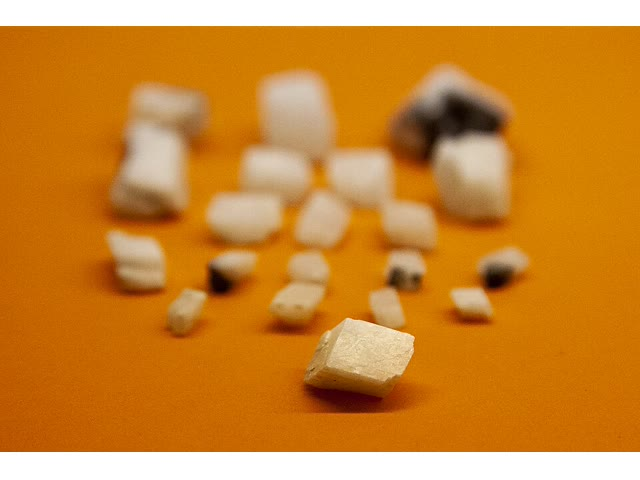
\includegraphics[width=\linewidth]{images/book3/b1-mineral-calcite-rhombs.jpg}

{\scriptsize Rhomboèdres de clivage de la calcite. Photographie Giovanna Canu et
Eva Santini, CC BY 4.0 (Wikimedia Commons).}
\end{minipage}
\end{inthelab}

\begin{omfigure}
\setlength{\tabcolsep}{2pt}
\begin{tabular}{ccc}
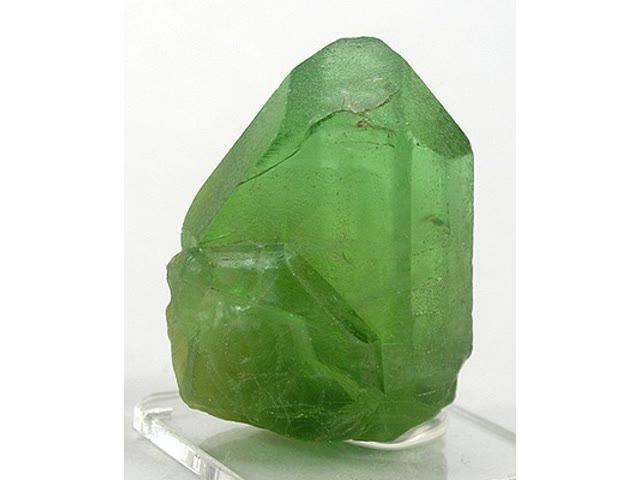
\includegraphics[width=0.31\linewidth]{images/book3/b1-mineral-olivine.jpg} &
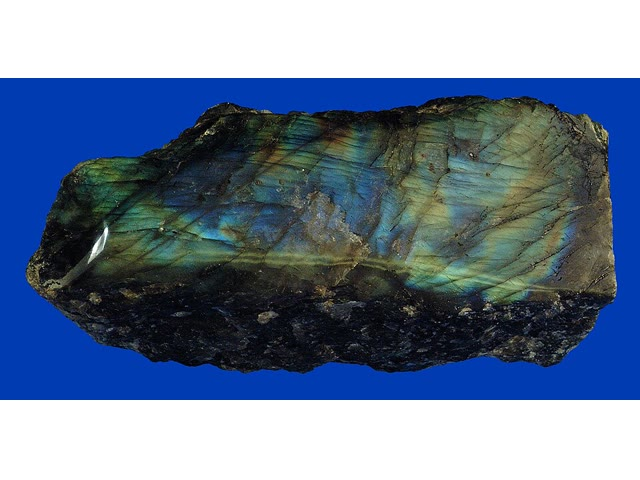
\includegraphics[width=0.31\linewidth]{images/book3/b1-mineral-plagioclase.jpg} &
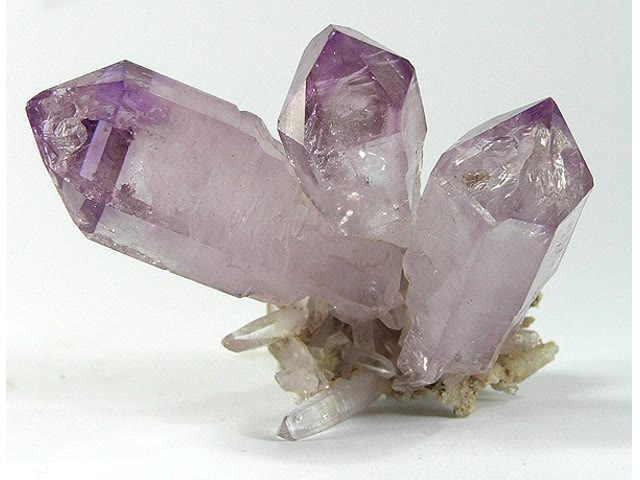
\includegraphics[width=0.31\linewidth]{images/book3/b1-mineral-quartz.jpg} \\
{\small (a) \omterm{def:b1:rock-forming-minerals:groups}{olivine}} & {\small (b) \omterm{def:b1:rock-forming-minerals:groups}{plagioclase} (labradorite)} & {\small (c) quartz (améthyste)} \\[4pt]
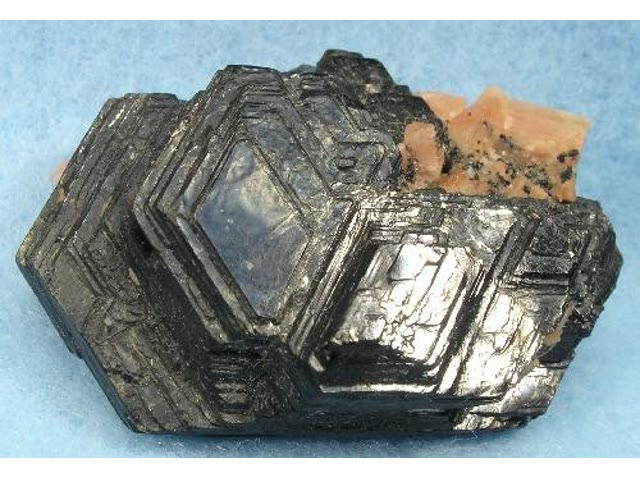
\includegraphics[width=0.31\linewidth]{images/book3/b1-mineral-biotite.jpg} &
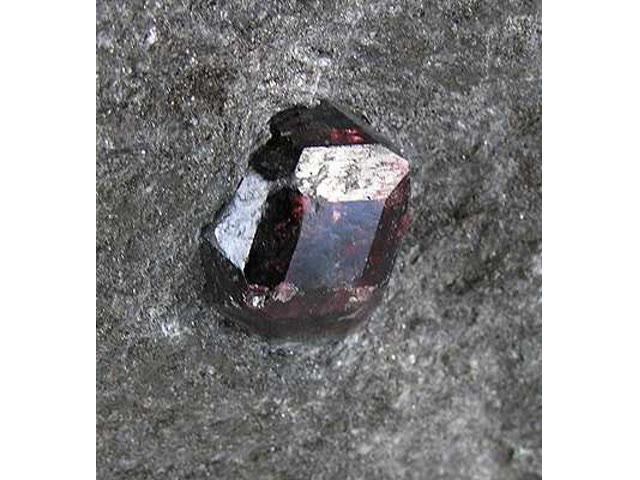
\includegraphics[width=0.31\linewidth]{images/book3/b1-mineral-garnet.jpg} &
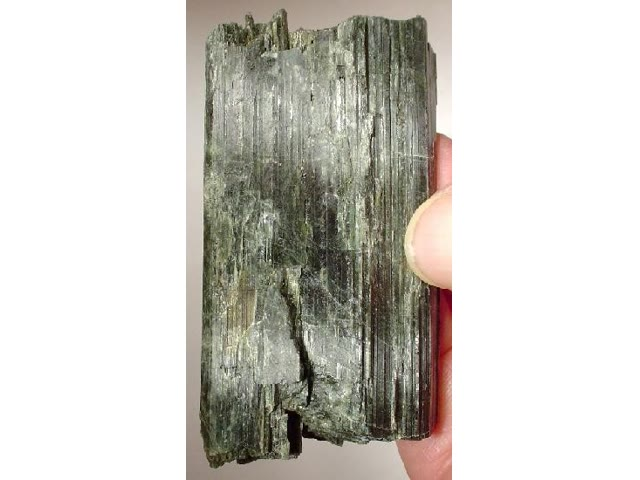
\includegraphics[width=0.31\linewidth]{images/book3/b1-mineral-hornblende.jpg} \\
{\small (d) biotite sur orthose} & {\small (e) \omterm{def:b1:rock-forming-minerals:groups}{grenat} (almandin)} & {\small (f) hornblende} \\
\end{tabular}
\medskip
% ledger: commons:min-olivine, commons:min-plagioclase, commons:min-quartz, commons:min-biotite, commons:min-garnet, commons:min-hornblende

{\small Six minéraux des roches~: (a) un cristal d'\omterm{def:b1:rock-forming-minerals:groups}{olivine} gemme~; (b) une dalle
polie de \omterm{def:b1:rock-forming-minerals:groups}{plagioclase} montrant le jeu de couleurs de la labradorite~; (c) des
cristaux de quartz, prismes à six pans à pointes pyramidales~; (d) un livre de
paillettes de biotite sur un cristal d'orthose~; (e) un cristal de \omterm{def:b1:rock-forming-minerals:groups}{grenat}
almandin dans sa matrice~; (f) un prisme de hornblende. Photographies (a),
(c)--(f) Robert M.~Lavinsky, CC BY-SA 3.0~; (b) Twyla Baker, CC0 (Wikimedia
Commons).}
\end{omfigure}

\section{Exercices}

\begin{exercise}[$\star$]\label{exo:b1:rock-forming-minerals:1}
Nommer la classe de silicate de chaque anion, et donner le nombre $s$ de sommets
partagés par chaque tétraèdre~: \ce{SiO4^{4-}}, \ce{Si2O7^{6-}},
\ce{Si6O18^{12-}}, \ce{Si2O5^{2-}}, \ce{SiO2}. À quelle classe \ce{SiO3^{2-}}
pourrait-il appartenir~?
\end{exercise}

\begin{exercise}[$\star$]\label{exo:b1:rock-forming-minerals:2}
Avec les masses atomiques O \num{15.999}, Si \num{28.085}, Mg \num{24.305} et
Fe \qty{55.845}{g.mol^{-1}}, calculer les masses molaires de la forstérite et de
la fayalite, puis leurs volumes molaires à partir des masses volumiques
\num{3.275} et \qty{4.392}{g.cm^{-3}}.
% ledger: ciaaw:O, ciaaw:Si, ciaaw:Mg, ciaaw:Fe, hom:forsterite, hom:fayalite
\end{exercise}

\begin{exercise}[$\star$]\label{exo:b1:rock-forming-minerals:3}
En coordinence six, les rayons sont \ce{Mg^{2+}} \qty{0.72}{\angstrom},
\ce{Fe^{2+}} \qty{0.78}{\angstrom}, \ce{Ni^{2+}} \qty{0.69}{\angstrom},
\ce{Mn^{2+}} \qty{0.83}{\angstrom} et \ce{Ca^{2+}} \qty{1.00}{\angstrom}.
Calculer l'écart de chacun au rayon de \ce{Mg^{2+}} en pour cent, et dire,
d'après les règles de Goldschmidt, lesquels peuvent remplacer librement le
magnésium dans l'\omterm{def:b1:rock-forming-minerals:groups}{olivine}.
% ledger: shannon:radii, goldschmidt:size
\end{exercise}

\begin{exercise}[$\star$]\label{exo:b1:rock-forming-minerals:4}
Le graphite et le diamant ont pour masses volumiques \num{2.16} et
\qty{3.51}{g.cm^{-3}}~; la calcite et l'aragonite \num{2.71} et
\qty{2.93}{g.cm^{-3}}. De combien pour cent la masse volumique augmente-t-elle
dans chaque changement~? Quel \omterm{def:b1:rock-forming-minerals:polymorph}{polymorphe} de chaque paire se forme à la plus haute
pression~?
% ledger: webmineral:polymorphs, hom:calcite
\end{exercise}

\begin{exercise}[$\star\star$]\label{exo:b1:rock-forming-minerals:5}
Écrire la \omterm{def:b1:rock-forming-minerals:formula}{formule structurale} du \omterm{def:b1:rock-forming-minerals:groups}{plagioclase} $\text{An}_{30}$ (\qty{30}{\percent}
des grands sites occupés par le calcium), et vérifier qu'elle est neutre.
\end{exercise}

\begin{exercise}[$\star\star$]\label{exo:b1:rock-forming-minerals:6}
Dans une chaîne double, la moitié des tétraèdres partagent deux sommets et la
moitié en partagent trois. Compter les oxygènes d'un groupe répété de quatre
tétraèdres directement sur le panneau (f) de la figure des enchaînements, et
vérifier la formule \ce{Si4O11^{6-}} donnée par la
\cref{prop:b1:rock-forming-minerals:si-o}.
\end{exercise}

\begin{exercise}[$\star\star$]\label{exo:b1:rock-forming-minerals:7}
Recalculer sur quatre oxygènes l'analyse d'\omterm{def:b1:rock-forming-minerals:groups}{olivine} \qty{40.20}{\percent}
de \ce{SiO2}, \qty{47.10}{\percent} de \ce{MgO}, \qty{12.20}{\percent} de \ce{FeO},
\qty{0.40}{\percent} de \ce{NiO} (masse molaire de \ce{NiO}
\qty{74.692}{g.mol^{-1}}).
Donner sa \omterm{def:b1:rock-forming-minerals:formula}{formule structurale}, la vérifier, et donner sa teneur en forstérite.
Montrer ensuite que la teneur en forstérite peut se trouver à partir des seuls
pourcentages de \ce{MgO} et de \ce{FeO}.
\end{exercise}

\begin{exercise}[$\star\star$]\label{exo:b1:rock-forming-minerals:8}
Vérifier que la muscovite \ce{KAl2(Si3Al)O10(OH)2} est neutre. Ses feuillets de
tétraèdres ont un aluminium pour trois silicium~: quelle charge cela donne-t-il
au feuillet par unité formulaire, et quel ion l'équilibre~?
\end{exercise}

\begin{exercise}[$\star\star$]\label{exo:b1:rock-forming-minerals:9}
Avec les volumes molaires \num{42.96} et \qty{46.40}{cm^3.mol^{-1}} et les
masses molaires \num{140.691} et \qty{203.771}{g.mol^{-1}}~: (a) calculer la
masse volumique de $\text{Fo}_{50}$ par mélange idéal, et la comparer à la
moyenne des masses volumiques des \omterm{def:b1:rock-forming-minerals:solid-solution}{pôles purs}~; (b) trouver la teneur en
forstérite d'une \omterm{def:b1:rock-forming-minerals:groups}{olivine} de masse volumique \qty{3.600}{g.cm^{-3}}.
\end{exercise}

\begin{exercise}[$\star\star\star$]\label{exo:b1:rock-forming-minerals:10}
Avec les notations de la \cref{prop:b1:rock-forming-minerals:ideal-mixing},
montrer que
\[
  \rho(x) - \bigl(x\rho_1 + (1 - x)\rho_2\bigr) =
  \frac{x(1 - x)(\rho_1 - \rho_2)(V_1 - V_2)}{V(x)} .
\]
En déduire que la masse volumique de l'\omterm{def:b1:rock-forming-minerals:groups}{olivine} est au-dessus de la droite entre
les \omterm{def:b1:rock-forming-minerals:solid-solution}{pôles purs}, et calculer l'écart en $\text{Fo}_{50}$.
\end{exercise}

\begin{exercise}[$\star\star\star$]\label{exo:b1:rock-forming-minerals:11}
Un \omterm{def:b1:rock-forming-minerals:groups}{plagioclase} de gabbro donne \qty{54.10}{\percent} de \ce{SiO2},
\qty{28.90}{\percent} de \ce{Al2O3}, \qty{11.20}{\percent} de \ce{CaO},
\qty{5.10}{\percent} de \ce{Na2O} et \qty{0.30}{\percent} de \ce{K2O} (masses
molaires \num{60.083}, \num{101.961}, \num{56.077}, \num{61.979},
\qty{94.195}{g.mol^{-1}}). Le recalculer sur huit oxygènes~; vérifier que les
sites tétraédriques (Si + Al) contiennent 4 atomes et le grand site
(Ca + Na + K) 1~; vérifier la \omterm{def:b1:rock-forming-minerals:substitution}{substitution couplée} en comparant $\mathrm{Al} - 1$
à Ca~; donner la teneur en anorthite $100\,\mathrm{Ca}/(\mathrm{Ca} +
\mathrm{Na} + \mathrm{K})$.
\end{exercise}

\begin{exercise}[$\star\star\star$]\label{exo:b1:rock-forming-minerals:12}
Une microsonde ne distingue pas \ce{Fe^{2+}} de \ce{Fe^{3+}} et rapporte tout le
fer sous forme de \ce{FeO}. (a) Montrer que la magnétite pure \ce{Fe3O4}, analysée
ainsi, totalise \qty{93.09}{\percent}. (b) Recalculer cette analyse sur quatre
oxygènes, et dire pourquoi le résultat est impossible pour un \omterm{def:b1:rock-forming-minerals:mineral}{minéral} à trois
cations pour quatre oxygènes. (c) Recalculer plutôt sur trois cations, et trouver
les nombres de \ce{Fe^{2+}} et de \ce{Fe^{3+}} en exigeant que la formule soit
neutre. (d) Réexprimer l'analyse en \ce{FeO} et \ce{Fe2O3}, et donner le nouveau
total.
\end{exercise}

\section{Problème~: Une olivine d'un basalte}

\begin{problem}[{Problème du week-end --- recalculer une analyse à la microsonde
d'une olivine, écrire et vérifier sa formule, et trouver sa composition, sa masse
volumique et sa masse dans un mètre cube de basalte}]
\label{pb:b1:rock-forming-minerals:1}
% invented analysis: figdata/bachelor-1/solid_solution.py (OLIVINE_WT); values: calc/ch07.py
% ledger: ciaaw:O, ciaaw:Si, ciaaw:Mg, ciaaw:Fe, ciaaw:Mn, ciaaw:Ni, ciaaw:Ca, hom:forsterite, hom:fayalite, shannon:radii
Les cristaux verts d'un basalte sont de l'\omterm{def:b1:rock-forming-minerals:groups}{olivine}. Une analyse à la microsonde de
l'un d'eux donne, en pourcentage en masse d'oxydes~:
\begin{center}
\small
\begin{tabular}{lcccccc}
\hline
oxide & \ce{SiO2} & \ce{FeO} & \ce{MnO} & \ce{MgO} & \ce{NiO} & \ce{CaO} \\
\% en masse & 39.50 & 16.53 & 0.23 & 43.32 & 0.20 & 0.22 \\
\hline
\end{tabular}
\end{center}
Les masses atomiques sont O \num{15.999}, Si \num{28.085}, Fe \num{55.845}, Mn
\num{54.938}, Mg \num{24.305}, Ni \num{58.693}, Ca \qty{40.078}{g.mol^{-1}}.
La forstérite a une masse volumique de \qty{3.275}{g.cm^{-3}} et la fayalite de
\qty{4.392}{g.cm^{-3}}.

\medskip
\noindent\textbf{Partie I --- Des oxydes aux cations.}
\begin{enumerate}
  \item Calculer les masses molaires des six oxydes.
  \item Calculer le total de l'analyse. Qu'aurait suggéré un total de
        \qty{97}{\percent}~?
  \item Calculer le nombre de moles de chaque oxyde dans \qty{100}{g} d'\omterm{def:b1:rock-forming-minerals:groups}{olivine}.
  \item Calculer les moles d'oxygène qu'ils contiennent, et leur somme.
  \item Calculer les moles de chaque cation.
  \item Calculer le facteur qui ramène les oxygènes à quatre.
  \item Donner le nombre d'atomes de chaque élément pour quatre oxygènes, à trois
        décimales.
\end{enumerate}

\medskip
\noindent\textbf{Partie II --- La formule structurale.}
\begin{enumerate}[resume]
  \item L'\omterm{def:b1:rock-forming-minerals:groups}{olivine} a un site tétraédrique et deux sites octaédriques pour quatre
        oxygènes. Calculer la somme des cations autres que le silicium, et
        comparer les deux totaux de sites à la formule idéale.
  \item Écrire la \omterm{def:b1:rock-forming-minerals:formula}{formule structurale} de l'\omterm{def:b1:rock-forming-minerals:groups}{olivine}.
  \item Vérifier que la formule est neutre, et expliquer pourquoi cette
        vérification, contrairement à celle de la question 8, n'aurait pas pu
        échouer.
  \item À l'aide des rayons ioniques (\ce{Mg^{2+}} \qty{0.72}{\angstrom},
        \ce{Fe^{2+}} \qty{0.78}{\angstrom}, \ce{Ni^{2+}}
        \qty{0.69}{\angstrom}, \ce{Mn^{2+}} \qty{0.83}{\angstrom},
        \ce{Ca^{2+}} \qty{1.00}{\angstrom}, tous en coordinence six), expliquer
        pourquoi le nickel est courant dans l'\omterm{def:b1:rock-forming-minerals:groups}{olivine} et le calcium rare.
  \item La sonde rapporte tout le fer sous forme de \ce{FeO}. Expliquer pourquoi
        le nombre total de cations trouvé à la question 7 montre que l'\omterm{def:b1:rock-forming-minerals:groups}{olivine} ne
        contient pas de \ce{Fe^{3+}} significatif.
\end{enumerate}

\medskip
\noindent\textbf{Partie III --- La composition.}
\begin{enumerate}[resume]
  \item Calculer la teneur en forstérite $\mathrm{Fo} = 100\,\mathrm{Mg}/(\mathrm{Mg} +
        \mathrm{Fe})$, à une décimale.
  \item Quel est le \omterm{def:b1:rock-forming-minerals:formula}{nombre de magnésium} de l'\omterm{def:b1:rock-forming-minerals:groups}{olivine}~? Pourquoi est-il égal ici à
        la teneur en forstérite~?
  \item Écrire l'\omterm{def:b1:rock-forming-minerals:groups}{olivine} comme une \omterm{def:b1:rock-forming-minerals:solid-solution}{solution solide} binaire
        $\mathrm{Fo}_x\mathrm{Fa}_{1-x}$, en ignorant Mn, Ni et Ca, et donner la
        proportion de ses sites octaédriques occupés par le fer.
  \item Montrer que la teneur en forstérite se calcule à partir des seuls
        pourcentages de \ce{MgO} et de \ce{FeO}, sans le facteur de la
        question 6, et le faire.
  \item Une \omterm{def:b1:rock-forming-minerals:groups}{olivine} qui a cristallisé plus tard dans la même lave contient
        \qty{40.5}{\percent} de \ce{MgO} et \qty{20.0}{\percent} de \ce{FeO}.
        Calculer sa teneur en forstérite. Quelle \omterm{def:b1:rock-forming-minerals:groups}{olivine} est la plus riche en
        fer~?
\end{enumerate}

\medskip
\noindent\textbf{Partie IV --- Masse volumique et masse.}
\begin{enumerate}[resume]
  \item Calculer les masses molaires et les volumes molaires de la forstérite et
        de la fayalite (volumes molaires à deux décimales).
  \item En prenant l'\omterm{def:b1:rock-forming-minerals:groups}{olivine} comme le binaire $\mathrm{Fo}_x\mathrm{Fa}_{1-x}$ de
        la question 15, avec $x$ arrondi à trois décimales, calculer sa masse
        molaire et son volume molaire par mélange idéal.
  \item En déduire sa masse volumique, à trois décimales.
  \item La comparer à l'interpolation en ligne droite entre les masses volumiques
        des \omterm{def:b1:rock-forming-minerals:solid-solution}{pôles purs}.
  \item Le basalte contient \qty{12}{\percent} d'\omterm{def:b1:rock-forming-minerals:groups}{olivine} en volume. Quelle masse
        d'\omterm{def:b1:rock-forming-minerals:groups}{olivine} un mètre cube de basalte contient-il~?
  \item Le basalte a une masse volumique de \qty{2.95}{g.cm^{-3}}. Quelle est la
        proportion d'\omterm{def:b1:rock-forming-minerals:groups}{olivine} en masse~?
  \item Quelle est la teneur en forstérite de l'\omterm{def:b1:rock-forming-minerals:groups}{olivine}, arrondie au pour cent
        entier~?
\end{enumerate}
\end{problem}
